\documentclass[11pt,oneside]{article}
\usepackage[utf8]{inputenc}
\usepackage[a4paper,top=2cm,left=2cm,right=2cm,bottom=2cm]{geometry}
\usepackage{import}
\usepackage[T1]{fontenc}
\usepackage[german,ngerman]{babel}
\usepackage[table]{xcolor}
\usepackage{amsthm, esvect}
\usepackage{mathtools}
\RequirePackage{amssymb, amsfonts, amsmath, latexsym, verbatim, xspace}
\usepackage{systeme}
\usepackage{multicol}
\usepackage{multirow}
\usepackage{framed}
\usepackage{array}
\usepackage{ragged2e}
\usepackage{graphicx}
\usepackage{pdflscape}
\usepackage{epstopdf}
\usepackage{booktabs}
\usepackage{pdfpages}
\usepackage{float} % Allows putting an [H] in \begin{figure} to specify the exact location of the figure
\usepackage{wrapfig} % Allows in-line images such as the example fish picture
\usepackage{tikz, graphicx} % tikz
\usepackage[position=top]{subfig}
\usepackage[bookmarks=true]{hyperref}%Links
\usepackage{enumerate}
\usepackage{enumitem}
\usepackage[german,ruled,vlined,linesnumbered,algosection]{algorithm2e}
\usepackage[labelfont=sf]{caption}
\usepackage{lmodern}
\usepackage{lscape}
\usepackage{tabularx}
\usepackage{systeme}
\usepackage{hhline}
\usepackage{subfiles}
\usepackage{stackengine}
\usepackage{setspace}
\usepackage{MnSymbol}
\usepackage{tcolorbox}
\usepackage{bbm}
\usepackage{url}
\usepackage{xparse}
\usepackage{sectsty}
\usepackage{array}
\usepackage{ragged2e}
\usepackage{listings} %Stellt Code-Snippets sauber dar

% definiert die Sprache
\selectlanguage{German}

% add command for different dates in Swiss fashion
\newcommand{\monthwordlong}[1]{\ifcase#1 \or Januar\or Februar\or März\or April\or Mai\or Juni\or Juli\or August\or September\or Oktober\or November\or Dezember\fi}
\newcommand{\monthwordshort}[1]{\ifcase#1\or Jan\or Feb\or Mar\or Apr\or Mai\or Jun\or Jul\or Aug\or Sept\or Okt\or Nov\or Dez\fi}
\newcommand{\datelong}{\number\day.\:\monthwordlong{\the\month}\:\number\year}
\newcommand{\dateshort}{\number\day.\:\monthwordshort{\the\month}\:\number\year}

% define color of links inside a text
\definecolor{linkblue}{RGB}{0, 0, 80}
\definecolor{plotblue}{RGB}{100, 100, 255}
\definecolor{myblue}{RGB}{8,164,214}
\definecolor{myred}{RGB}{143,42,41}
\definecolor{forestgreen}{RGB}{34,139,34}
\definecolor{highdive}{RGB}{10,169,194}
\definecolor{charcoal}{RGB}{74,74,74}
\hypersetup{
	colorlinks=true,
	linkcolor=linkblue,
	filecolor=magenta,
	urlcolor=plotblue,
	citecolor=linkblue,
	pdfpagemode=FullScreen,
}


\lstdefinestyle{mystyle}{ % definiert den style des Code-Snippets
	%backgroundcolor=\color{backcolour},
	%commentstyle=\color{codegreen},
	%keywordstyle=\color{magenta},
	%numberstyle=\tiny\color{codegray},
	%stringstyle=\color{codepurple},
	basicstyle=\ttfamily\footnotesize,
	breakatwhitespace=false,
	breaklines=true,
	captionpos=b,
	keepspaces=true,
	%numbers=left,
	%numbersep=5pt,
	showspaces=false,
	showstringspaces=false,
	showtabs=false,
	tabsize=4
}
\lstset{style=mystyle}
\usepackage{fancyhdr}

\tcbuselibrary{breakable,skins}
\usetikzlibrary{mindmap,trees}
\newlength\tindent
\setlength{\tindent}{\parindent}
\setlength{\parindent}{0pt}
\renewcommand{\indent}{\hspace*{\tindent}}

\makeatletter
\def\ifEmpty#1{\def\@temp{#1}\ifx\@temp\@empty}
\makeatother

\sectionfont{\underline}
\usetikzlibrary{arrows, petri, topaths, graphs}


% =================== BEISPIEL ====================
\theoremstyle{definition}
\newtheorem{beispiel}{Beispiel}
\renewcommand{\thebeispiel}{\arabic{beispiel}}

% =================== AUFGABE =====================
\newcounter{aufg}[section] % Zähler für die Umgebungen

\newenvironment{aufgabe}[1][]{%
    \refstepcounter{aufg}% Inkrementiere den Zähler
    \begin{tcolorbox}[%
        enhanced,
        overlay unbroken and first={\mytitleaufg[#1]}, % Titelleiste mit Icons wird nicht über Seite gebrochen
        colframe=black,
        boxrule=0pt,
        breakable,
        top=15pt,
        before=\vskip18pt,
    ]
}{%
    \end{tcolorbox}
}

\newcommand{\mytitleaufg}[1][]{% Definiert die Titelleiste und Icons
    \node[fill=black!20,
        rounded corners,
        draw=black,
        text=black,
        line width=1pt,
        inner sep=4pt,
        anchor=west,
        xshift=12pt]
        at (frame.north west){\bfseries Aufgabe \thesection.\theaufg.\ifEmpty{#1}\else\emph{ (#1)}\fi}; % Titel, letzter Teil mit ifempty testet ob #1 leer und macht Klammern und Titel, falls Titelargument übergeben wird bzw. falls #1 leer erscheint nichts - auch keine Klammern

    \node[% Icon
        rounded corners,
        text=black,
        fill=black,
        line width=0pt,
        inner sep=3pt,
        anchor=west,
        xshift=5pt,
        % yshift=-35pt
        ]
        at (frame.north east){
\includegraphics[width=24pt]{../../../Header/Icons/aufgabeicon.png}};
}

% =================== DEFINITION ==================
\newcounter{def}[section] % Zähler für die Umgebungen

\newenvironment{definition}[1][]{%
    \refstepcounter{def}% Inkrementiere den Zähler
    \begin{tcolorbox}[%
        enhanced,
        drop shadow southeast,
        overlay unbroken and first={\mytitledef[#1]}, % Titelleiste mit Icons wird nicht über Seite gebrochen
        colback=blue!5!white,
        colframe=blue!75!black,
        boxrule=2pt,
        breakable,
        top=15pt,
        before=\vskip18pt,
    ]
}{%
    \end{tcolorbox}
}

\newcommand{\mytitledef}[1][]{% Definiert die Titelleiste und Icons
    \node[fill=blue!40!white,
        rounded corners,
        draw=black,
        text=black,
        line width=1pt,
        inner sep=4pt,
        anchor=west,
        xshift=12pt]
        at (frame.north west){\bfseries Definition \thesection.\thedef.\ifEmpty{#1}\else\emph{ (#1)}\fi}; % Titel, letzter Teil mit ifempty testet ob #1 leer und macht Klammern und Titel, falls Titelargument übergeben wird bzw. falls #1 leer erscheint nichts - auch keine Klammern

    \node[% Icon
        rounded corners,
        text=black,
        fill=black,
        line width=0pt,
        inner sep=3pt,
        anchor=west,
        xshift=5pt,
        % yshift=-35pt
        ]
        at (frame.north east){
\includegraphics[width=24pt]{../../../Header/Icons/definitionicon.png}};
}

% =================== NOTATION ====================
\newcounter{nota}[section] % Zähler für die Umgebungen

\newenvironment{notation}[1][]{%
    \refstepcounter{nota}% Inkrementiere den Zähler
    \begin{tcolorbox}[%
        enhanced,
        drop shadow southeast,
        colback=yellow!5!white,
        colframe=yellow!75!black,
        overlay unbroken and first={\mytitlenota[#1]},   % Titelleiste mit Icons wird nicht über Seite gebrochen
        boxrule=2pt,
        breakable,
        top=15pt,
        before=\vskip18pt,
    ]
}{%
    \end{tcolorbox}
}

\newcommand{\mytitlenota}[1][]{% Definiert die Titelleiste und Icons
    \node[fill=yellow!40!white,,
        rounded corners,
        draw=black,
        text=black,
        line width=1pt,
        inner sep=4pt,
        anchor=west,
        xshift=12pt]
        at (frame.north west){\bfseries Notation \thesection.\thenota.\ifEmpty{#1}\else\emph{ (#1)}\fi}; % Titel, letzter Teil mit ifempty testet ob #1 leer und macht Klammern und Titel, falls Titelargument übergeben wird bzw. falls #1 leer erscheint nichts - auch keine Klammern

    \node[% Icon
        rounded corners,
        text=black,
        fill=black,
        line width=0pt,
        inner sep=3pt,
        anchor=west,
        xshift=5pt,
        % yshift=-35pt
        ]
        at (frame.north east){
\includegraphics[width=24pt]{../../../Header/Icons/definitionicon.png}};
}

% =================== SATZ ========================
\newcounter{satz}[section]  % creates a counter and resets it after each chapter

\newenvironment{satz}[1][]{   % Hauptbox mit Satz drin
    \refstepcounter{satz}
    \begin{tcolorbox}[%
        enhanced,
        colback=red!5!white,
        fuzzy halo=2mm with gray,
        colframe=red!75!black,
        overlay unbroken and first={\mytitlesatz[#1]},   % Titelleiste mit Icons wird nicht über Seite gebrochen
        boxrule=2pt,
        breakable,
        top=15pt,
        before=\vskip18pt,
    ]
}{%
    \end{tcolorbox}
}

\newcommand{\mytitlesatz}[1][]{                     % Macht Titelbox und Icons
   \node[fill=red!90!white,
      rounded corners,
      draw=black,,
      text=black,
      line width=1pt,
      inner sep=4pt,
      anchor=west,
      xshift=12pt]
   at (frame.north west){\bfseries Satz \thesection.\thesatz.\ifEmpty{#1}\else\emph{ (#1)}\fi};  % Titel, letzter Teil mit ifx testet ob #1 leer und macht Klammern und Titel, falls Titelargument übergeben wird bzw.  falls #1 leer erscheint nichts - auch keine Klammern

 \node[ % Icon
      rounded corners,
      text=black,
      fill=black,
      line width=0pt,
      inner sep=3pt,
      anchor=west,
      xshift=5pt,
%     yshift=-35pt
]
   at (frame.north east){ 
\includegraphics[width=24pt]{../../../Header/Icons/satzicon.png} };
}

% =================== BEWEIS ======================
\newenvironment{beweis}[1][]{
    \begin{tcolorbox}[
        enhanced,
        overlay unbroken and first={\mybeweis[#1]},     % Titelleiste mit Icons wird nicht über Seite gebrochen
        colback=white,
        colframe=black,
        boxrule=0pt,
        breakable,
        top=15pt,
        before=\vskip18pt,
    ]
}{
        \end{tcolorbox}
}

\newcommand{\mybeweis}[1][]{                     % Macht Titelbox und Icons
   \node[fill=white,
      rounded corners,
      draw=black,
      text=black,
      line width=1pt,
      inner sep=4pt,
      anchor=west,
      xshift=12pt]
   at (frame.north west){\bfseries Beweis \ifEmpty{#1}\else\emph{ (#1)}\fi};  % Titel, letzter Teil mit ifx testet ob #1 leer und macht Klammern und Titel, falls Titelargument übergeben wird bzw.  falls #1 leer erscheint nichts - auch keine Klammern
}

% =================== ALGORITHM ===================
\newcounter{algo}[section]  % creates a counter and resets it after each chapter

\newenvironment{algo}[1][]{   % Hauptbox mit Satz drin
    \refstepcounter{algo}
    \begin{tcolorbox}[%
        enhanced,
        drop shadow southeast,
        colback=yellow!5!white,
        colframe=yellow!75!black,
        overlay unbroken and first={\algotitle[#1]},   % Titelleiste mit Icons wird nicht über Seite gebrochen
        boxrule=2pt,
        breakable,
        top=15pt,
        before=\vskip18pt,
    ]
}{%
    \end{tcolorbox}
}

\newcommand{\algotitle}[1][]{                     % Macht Titelbox und Icons
   \node[fill=yellow!40!white,
      rounded corners,
      draw=black,
      text=black,
      line width=1pt,
      inner sep=4pt,
      anchor=west,
      xshift=12pt]
   at (frame.north west){\bfseries \ifEmpty{#1}{Ablauf}\else{#1}\fi};  % Titel, letzter Teil mit ifx testet ob #1 leer und macht Klammern und Titel, falls Titelargument übergeben wird bzw.  falls #1 leer erscheint nichts - auch keine Klammern

 \node[ % Icon
      rounded corners,
      text=black,
      fill=black,
      line width=0pt,
      inner sep=3pt,
      anchor=west,
      xshift=5pt
      % yshift=-35pt
      ]
   at (frame.north east){ 
\includegraphics[width=24pt]{../../../Header/Icons/algoicon.png} };
}

% ================ Nummerierte Multicol ================
\newenvironment{enumcols}[1][]{
    \begin{enumerate}[label=\alph*)]\begin{multicols}{#1}
}{
    \end{multicols}\end{enumerate}
}



% =================================================
\usetikzlibrary{shapes,arrows}
\tikzstyle{decision} = [diamond, draw, fill=blue!20,
    text width=6em, text badly centered, node distance=4cm, inner sep=0pt]
\tikzstyle{block} = [rectangle, draw, fill=blue!20,
    text width=8em, text centered, rounded corners, minimum height=4em]
\tikzstyle{line} = [draw, -latex']
\tikzstyle{cloud} = [draw, ellipse,fill=red!20, node distance=2cm,
    minimum height=2em]

% Karriertes Papier für Antwort
\newcommand{\karos}[1]{\begin{tikzpicture}\draw[step=0.5cm,color=gray] (0,0) grid (\linewidth,#1 cm);\end{tikzpicture}}
%%
% Header and Footer
%%
\linespread{1.2} % Line spacing
\fancypagestyle{plain}{
	\pagestyle{fancy}
	\lhead{}
	\chead{}
	\rhead{}
	\lfoot{\Autor}
	\cfoot{\Skriptname}
	\rfoot{\thepage}
	\renewcommand{\headrulewidth}{0pt}
	\renewcommand{\footrulewidth}{0.4pt}
}

\pagestyle{fancy}
\fancyhf{}
\rhead{\rightmark}
\lfoot{\leftmark}
\rfoot{\thepage}
\renewcommand{\headrulewidth}{0.2pt}
%\setlength\parindent{0pt} % Uncomment to remove all indentation from paragraphs



%%
% Math Arrows
%%
\newcommand{\same}{\ensuremath{\Longleftrightarrow}}
\renewcommand{\to}{\ensuremath{\longrightarrow}}
\newcommand{\qsame}{\quad\same\quad}
\newcommand{\dsame}{\ensuremath{:\Leftrightarrow}}
\newcommand{\qdsame}{\quad\dsame\quad}
\newcommand{\ldsame}{\ensuremath{:\Longleftrightarrow}}
\newcommand{\samedef}{\ensuremath{\us {\text{def}} \Leftrightarrow}}
\newcommand{\qsamedef}{\quad\samedef\quad}
\newcommand{\lsamedef}{\ensuremath{\us {\text{def}} \Longleftrightarrow}}
\newcommand{\qlsamedef}{\quad\lsamedef\quad}


%%
% Mengendefinitionen
%%
\newcommand{\M}{\ensuremath{\mathcal{M}}}
\newcommand{\N}{\ensuremath{\mathbb{N}}}
\newcommand{\Z}{\ensuremath{\mathbb{Z}}}
\newcommand{\Q}{\ensuremath{\mathbb{Q}}}
\newcommand{\I}{\ensuremath{\mathbb{I}}}
\newcommand{\R}{\ensuremath{\mathbb{R}}}
\newcommand{\C}{\ensuremath{\mathbb{C}}}
\renewcommand{\S}{\ensuremath{\mathbb{S}}}
\newcommand{\Prim}{\ensuremath{\mathbb{P}}}
\newcommand{\0}{\ensuremath{\emptyset}}
\renewcommand{\Re}{\ensuremath{\operatorname{Re}}}
\renewcommand{\Im}{\ensuremath{\operatorname{Im}}}
\newcommand{\strich}{\ensuremath{\big\vert}}

%%
% Mengenoperation
%%
\renewcommand{\nin}{\not\in}


%%
% Logisches Und und Oder
%%
\newcommand{\sand}{\ensuremath{\; \land \;}}
\newcommand{\sor}{\ensuremath{\; \lor \;}}
\renewcommand{\*}{\ensuremath{\cdot}}
\newcommand{\oder}{\vee}
\newcommand{\n}{\neg}
\newcommand{\und}{\wedge}


%%
% Bei Integral, Summe,... die Grenzen über bzw.
% unter das Zeichen
%%
\renewcommand{\d}[1]{\ensuremath{\operatorname{d}\!{#1}}}
\newcommand{\Sum}{\sum\limits}
\newcommand{\Prod}{\prod\limits}
\newcommand{\Min}{\min\limits}
\newcommand{\Max}{\max\limits}
\newcommand{\Lim}{\lim\limits}
\newcommand{\Inf}{\inf\limits}
\newcommand{\Sup}{\sup\limits}
\newcommand{\Liminf}{\liminf\limits}
\newcommand{\Limsup}{\limsup\limits}
%\renewcommand{\Cup}{\bigcup\limits}
%\renewcommand{\Cap}{\bigcap\limits}
\newcommand{\Otimes}{\bigotimes\limits}
\newcommand{\Oplus}{\bigoplus\limits}


%%
% Arcus Cotangens, Logarithmus
%%
\let\oldsin\sin
\renewcommand{\sin}[1]{\oldsin{\left(#1\right)}}
\let\oldcos\cos
\renewcommand{\cos}[1]{\oldcos{\left(#1\right)}}
\let\oldtan\tan
\renewcommand{\tan}[1]{\oldtan{\left(#1\right)}}
\let\oldarcsin\arcsin
\renewcommand{\arcsin}[1]{\oldarcsin{\left(#1\right)}}
\let\oldarccos\arccos
\renewcommand{\arccos}[1]{\oldarccos{\left(#1\right)}}
\let\oldarctan\arctan
\renewcommand{\arctan}[1]{\oldarctan{\left(#1\right)}}
\let\oldln\ln
\renewcommand{\ln}[1]{\oldln{\left(#1\right)}}
\newcommand{\Log}[2]{\ensuremath{\operatorname{log}_{#1}\left(#2\right)}}
\newcommand{\e}{\operatorname{e}}
\renewcommand{\exp}[1]{\ensuremath{\operatorname{\e}^{#1}}}


%%
% Griechische Buchstaben
%%
\renewcommand{\epsilon}{\ensuremath{\varepsilon}}
\renewcommand{\phi}{\varphi}
\renewcommand{\l}{\lambda}
\renewcommand{\t}{\tau}


%%
% Bezeichnungen
%%
\newcommand{\Rgn}{\R_{>0}} % R grösser Null
\newcommand{\Rad}{\operatorname{Rad}}   % Radikal
\newcommand{\kgV}{\operatorname{kgV}}   % Kleinster gemeinsame Vielfache
\newcommand{\ggT}{\operatorname{ggT}}   % Grösster gemeinsame Teiler
\newcommand{\winkel}{\sphericalangle}          % Winkelsymbol
\DeclarePairedDelimiter\abs{\lvert}{\rvert} % besserer Betrag
\makeatletter
\let\oldabs\abs
\def\abs{\@ifstar{\oldabs}{\oldabs*}}
\makeatother


%%
% Vektorgeometrie
%%
\renewcommand{\v}[1]{\vv{#1}}       % besserer Pfeil über Buchstaben
\renewcommand{\vec}[2]{\begingroup\renewcommand{\arraystretch}{1}\left(\begin{array}{c} #1 \\ #2 \end{array}\right)\endgroup}   % two dimensional vector
\renewcommand{\Vec}[3]{\begingroup\renewcommand{\arraystretch}{1}\left(\begin{array}{c} #1 \\ #2 \\ #3 \end{array}\right)\endgroup}      % three dimensional vector


%%
% Text
%%
\newcommand*{\Ueq}[1]{\mathrel{\mathop{=}\limits_{\text{#1}}}}
\newcommand*{\Oeq}[1]{\mathrel{\stackrel{\text{#1}}{=}}}
\newcommand{\utext}[2]{\underbrace{#1}_{\substack{#2}}}
\newcommand{\otext}[2]{$\overbrace{\textrm{#1}}^{\textrm{#2}}$}
\newcommand{\lineortext}[1]{\hspace{0,1cm}\underline{\hspace{0.1cm}\hphantom{#1}\hspace{0.1cm}}\hspace{0,1cm}} % Lückentext erstellen
\newcommand{\gap}[1]{\rule{#1 cm}{1pt}}


\newcommand{\Skriptname}{Rationale Potenzen}
\newcommand{\Autor}{Jonas Guler (Gu)}
\newcommand{\version}{\textit{v}1.0}

\begin{document}   %KSH-Gubser - LATEX/PDF
\begin{titlepage}
	\clearpage
	\title{\Huge\textbf{\Skriptname} \\[1cm]}
	\author{Autor:\\ \Autor}
	\date{\normalsize {Version \version}\\ \datelong}
	\maketitle
	\thispagestyle{empty}
	\vfill
	\tableofcontents
\end{titlepage}
\pagenumbering{arabic}
%############################################################################################
\section{Potenzen mit negativen Exponenten}
Im ersten Kanti-Jahr habe wir die folgenden Potenzgesetze kennengelernt.
\begin{satz}[Potenzgesetze für natürliche Exponenten]
	Für Potenzen mit reellen Basen $a,b\in\R$ und natürlichen Exponenten $m,n\in\N $ gelten folgende Rechengesetze:
	\begingroup
	\renewcommand{\arraystretch}{2}
	\begin{table}[H]
		\centering
		\begin{tabular}{l c}
			Potenzen mit gleicher Basis & $\displaystyle a^{m}\*a^{n}=a^{m+n}$ \\
			Potenzen mit gleichem Exponenten & $\displaystyle a^{n}\*b^{n}=(ab)^n$ \\
			Verschachtelte Potenzen & $\displaystyle(a^{m})^{n}=a^{m\*n}$ \\
			Potenz eines Bruches mit gleicher Basis & $\displaystyle\frac{a^m}{a^n}=a^{m-n}$ \\
			Potenz eines Bruches mit gleichem Exponent & $\displaystyle\frac{a^n}{b^n}=\left(\frac{a}{b}\right)^n$ \\
		\end{tabular}
	\end{table}
	\endgroup
	Es liegt auf der Hand, dass bei 4. $a\neq0$ und bei 5. $b\neq0$ gelten muss.
\end{satz}
Wenden wir diese direkt in einer Repetitionsaufgabe an.
\begin{aufgabe}
	Bob, Alice und Carol beschäftigen sich mit Potenzen. Sie sind bei den folgenden Aufgaben jedoch nicht einer Meinung, was die Lösungen angehen. Wer ist jeweils korrekt? Begründe anhand der Potenzgesetze.
	\begin{enumerate}[label=\alph*)]
		\item$2^7\*2^{10}=$\begin{enumerate}\begin{multicols}{3}
				\item[Alice: ] $2^{17}$
				\item[Bob: ] $2^{70}$
				\item[Carol: ] $4^{70}$
		\end{multicols}\end{enumerate}
		\item$3^5\*7^5=$\begin{enumerate}\begin{multicols}{3}
				\item[Alice: ] $21^{10}$
				\item[Bob: ] $21^{25}$
				\item[Carol: ] $21^{5}$
		\end{multicols}\end{enumerate}
		\item$\left(3^4\right)^5=$\begin{enumerate}\begin{multicols}{3}
				\item[Alice: ] $3^{9}$
				\item[Bob: ] $3^{20}$
				\item[Carol: ] $3^{\left(4^5\right)}$
		\end{multicols}\end{enumerate}
		\item$\frac{12^5}{3^5}=$\begin{enumerate}\begin{multicols}{3}
				\item[Alice: ] $9^{5}$
				\item[Bob: ] $\left(\frac{12}{3}\right)^5$
				\item[Carol: ] $4^5$
		\end{multicols}\end{enumerate}
	\end{enumerate}
	\karos{3}
\end{aufgabe}
Beachte, dass im Potenzgesetz 4. gefordert wird, dass $n>m$, weil wir ansonsten einen negativen Exponenten erhalten würden. Genau diesem Problem möchten wir nun auf die Spur begeben und genauer unter die Lupe nehmen. Starten wir mit einem Beispiel: \[2^5\div2^8=\gap{2}.\]
Was bedeutet aber $2^{-3}$? Was für eine Zahlenwert hat dieser Term?
\begin{figure}[H]
	\centering
	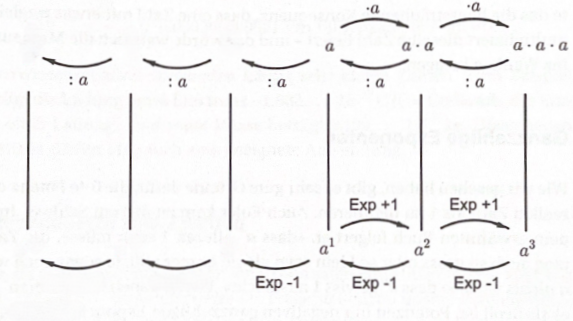
\includegraphics[scale=0.8]{images/ganzzahligeexp.png}
\end{figure}
Aus der obigen Graphik lassen sich die folgenden beiden Definitionen ablesen.
\begin{definition}
	Sei $a\in\R$ eine beliebige reelle Zahl und $n\in\Z$ eine beliebige ganze Zahl. Dann gilt:
	\begin{enumerate}[label=\ ]\begin{multicols}{2}
			\item $a^0=1$ \item $\displaystyle a^{-n}=\frac{1}{a^n}$
	\end{multicols}\end{enumerate}
\end{definition}
Natürlich muss im Punkt 2. die Einschränkung $a\neq0$ ebenfalls gelten, anderenfalls wäre der Bruch natürlich nicht definiert. Selbstverständlich lassen sich alle Potenzgesetze auf ganzzahlige Exponenten erweitern. Um dies aufzuzeigen, möchten wir das erste Gesetz auch für zwei negative negative Exponenten beweisen.\newline
Wir behaupten $\mathbf{a^n\*a^m=a^{n+m}}$ für eine beliebige reelle Zahl $a$ und zwei negative Exponenten $n$ und $m$.
\begin{beweis}
	\karos{4}
\end{beweis}
\begin{aufgabe}
	BlaBlaBla
\end{aufgabe}

\newpage
\section{Die n-te Wurzeln}



\begin{definition}
	Sei $a\in\R_0^+$ und $n\in\N$. Die \textbf{n-te Wurzel} von $a$ ist diejenige nicht-negative reele Zahl $x$, sodass \[\lineortext{x^n=a}\] gilt. Wir schreiben auch $x=\sqrt{a}$. Der Term unter der Wurzel heisst \textit{Radikand}.
	Falls $n=2$ gilt, handelt es sich um die bereits bekannte Quadratwurzel, wobei man meistens den Wurzelindex weglässt: \[\sqrt[2]{a}=\sqrt{a}.\]
\end{definition}

\subsection{Wurzeln als rationale Exponenten}

\subsection{Anwendungen}
\subsubsection{Lineare Gleichungen mit Wurzelkoeffizienten}
Als erstes betrachten wir die bereits bekannten linearen Gleichungen, aber wir lassen als Koeffizienten auch Wurzelterme zu. Dass heisst, der Faktor vor der Unbekannten kann eine Wurzel enthalten. Der Lösungsweg geht genau gleich wie ohne Wurzel. Zur Erinnerung fassen wir nochmals zusammen:
\begin{algo}
	\begin{enumerate}
		\item ausmultiplizieren, falls notwendig
		\item alle Unbekannte auf die eine Seite, der Rest auf die andere Seite
		\item die Unbekannte ausklammern
		\item durch die Klammer vor der Unbekannten dividieren
	\end{enumerate}
\end{algo}
Starten wir mit einem Beispiel gemeinsam.
\begin{beispiel}
	\[x\sqrt{8}+6=\sqrt{8}-x\]
	\karos{4}
\end{beispiel}
\begin{aufgabe}
	Löse die linaeren Gleichungen nach $x$ auf.
	\begin{enumerate}[label=\alph*)]\begin{multicols}{2}
			\item $x\sqrt{2}+\sqrt{3}=\sqrt{5}-x\sqrt{2}$
			\item $4x-5=\sqrt{6}\cdot x+7$
			\item $(x-4)\sqrt{2}=\sqrt{3}(x-5)$
			\item $(x+2-\sqrt{2})^2=x^2+\sqrt{2}$
	\end{multicols}\end{enumerate}
\end{aufgabe}
\subsubsection{Quadrierte Gleichungen}
Als erste Anwendung betrachten wir eine neue Form von Gleichungen, die wir allerdings mit einem Trick auf die linearen Gleichungen zurückführen können. Das heisst auch, die Unbekannte ist nie unter der Wurzel anzutreffen.
\begin{definition}
	Eine Gleichung heisst quadrierte Gleichung, falls die Unbekannte im Quadrat vorkommt.
\end{definition}
Starten wir mit zwei gemeinsamen Beispielen:
\begin{beispiel}\begin{enumerate}
		\item \[(x-3)^2=64\]\karos{6}\newpage
		\item \[(3x-16)^2=(4x-19)^2\]\karos{6}
\end{enumerate}\end{beispiel}
\begin{aufgabe}
	Löse die folgenden Gleichungen. Überlege dir genau welche beiden Fälle du betrachten musst.
	\begin{enumerate}[label=\alph*)]\begin{multicols}{2}
			\item $(x-6)^2=(2x-7)^2$
			\item $(2x+3)^2-9\*(6x-7)^2=16\*(6x-7)^2$
			\item $9x^4=(5x^2-2)^2$
			\item $(x^2+x-14)^2=(x^2-x+6)^2$
	\end{multicols}\end{enumerate}
\end{aufgabe}
\subsubsection{Wurzelgleichungen}
Als zweites betrachten wir sogenannte Wurzelgleichungen. Diese zeichnen sich aus, dass die Unbekannte unter der Wurzel zu finden ist. Um die Gleichung lösen zu können, müssen wir es schaffen, die Unbekannte aus der Wurzel herausnehmen zu können.
\begin{beispiel}
	\[x+1=\sqrt{2x+5}\]\karos{4}
\end{beispiel}
\textbf{Wichtig: } Durch das \lineortext{quadrieren} einer Gleichung können zusätzliche falsche Lösungen entstehen. Deshalb ist eine Überprüfung der Lösungen unerlässlich.\newline
\karos{2}
\begin{aufgabe}
	Löse die folgenden Gleichung nach $x$ auf und überprüfe sie hinsichtlich möglicher Scheinlösungen.
	\begin{enumerate}[label=\alph*)]\begin{multicols}{2}
			\item $\sqrt{x+5}=\sqrt{4-x}$
			\item $\sqrt{x(x-4)}=2\sqrt{1-x}$
			\item $\sqrt{3x^2-50}=-x$
			\item $\sqrt{x}+\sqrt{x+4}=4$
			\item $\sqrt{6-x}+\sqrt{2x+1}=\sqrt{x+7}$
			\item $\sqrt{x-2}+\sqrt{x-11}=\sqrt{x+13}$
	\end{multicols}\end{enumerate}
\end{aufgabe}

\newpage
\subsection*{History}
\begin{table}[H]
	\centering
	\begin{tabular}{|p{13mm}|p{20mm}|p{30mm}|p{70mm}|}\hline
		%\multicolumn{4}{|l|}{History}\\\hline
		Version & Datum & Person & Bemerkung \\\hline
		$0.1$ & 16.12.2023 & Jonas Guler & Kapitel erstellt \\\hline
		$0.2$ & 02.10.2024 & Jonas Guler & Definition auf n-te Wurzel verallgemeinert \\\hline
		$0.3$ & ToDo & Jonas Guler & Aufgaben hinzufügen und Rationale Exponenten \\\hline
	\end{tabular}
\end{table}



\end{document}
